\documentclass[../../main.tex]{subfiles}
\graphicspath{{../../image/}{../../figure/}}
\begin{document}

\section{记号与假设}\label{section:ch12-记号与假设}

我们考虑一个真非线性、严格双曲的两方程守恒律组，
\begin{align}
\partial_t U(x,t)+\partial_x F(U(x,t))=0,
\label{align:ch12-系统}
\end{align}
定义在以原点为中心的某个圆盘 $\mathscr{O}$ 上。$DF$ 的特征值（特征速度）在此记为 $\lambda$ 与 $\mu$，满足 $\lambda(U)<0<\mu(U)$（$U\in\mathscr{O}$），相应的特征向量记为 $R$ 与 $S$。

该系统配有一个 Riemann 不变量的坐标系 $(z,w)$，它在原点 $U=0$ 处取零值，并按原书 (7.3.8) 归一化：
\begin{align}
\mathrm{D}_z R=1,\qquad \mathrm{D}_z S=0,\qquad \mathrm{D}_w R=0,\qquad \mathrm{D}_w S=1.
\label{align:ch12-riemann归一}
\end{align}
真非线性条件现由原书 (7.5.4) 给出，在此即
\begin{align}
\lambda_z<0,\qquad \mu_w>0.
\label{align:ch12-真非线性}
\end{align}
不等式\eqref{align:ch12-真非线性}方向的选取，使得 $z$ 跨过可容许弱 1-激波时增大，而 $w$ 跨过可容许弱 2-激波时减小。

为确定起见，我们考虑这样一类系统：任意两个同族激波的相互作用产生一个同族激波和一个异族稀疏波。注意，这一条件在此由下式表达：
\begin{align}
S^{\top}\mathrm{D}^2_z S>0,\qquad R^{\top}\mathrm{D}^2_w R>0.
\label{align:ch12-相互作用}
\end{align}
事实上，结合原书 (8.2.24)、\eqref{align:ch12-真非线性} 与原书定理 8.3.1，不等式\eqref{align:ch12-相互作用}蕴含：$z$ 跨过可容许弱 2-激波时增大，而 $w$ 跨过可容许弱 1-激波时减小。
因此，从状态 $(\bar z,\bar w)$ 发出的可容许激波曲线与稀疏波曲线具有\cref{figure:ch12-激波稀疏曲线}所示的形状。于是，如\cref{figure:ch12-激波相互作用}(a) 所示，一个连接左状态 $(z_\ell,w_\ell)$ 与右状态 $(z_m,w_m)$ 的 2-激波，与一个连接左状态 $(z_m,w_m)$ 与右状态 $(z_r,w_r)$ 的 2-激波相互作用，产生一个连接左状态 $(z_\ell,w_\ell)$ 与右状态 $(z_0,w_\ell)$ 的 1-稀疏波，以及一个连接左状态 $(z_0,w_\ell)$ 与右状态 $(z_r,w_r)$ 的 2-激波，如\cref{figure:ch12-激波相互作用}(b) 所示。类似地，两个 1-激波的相互作用产生一个 1-激波和一个 2-稀疏波。

\begin{figure}[ht]
\centering
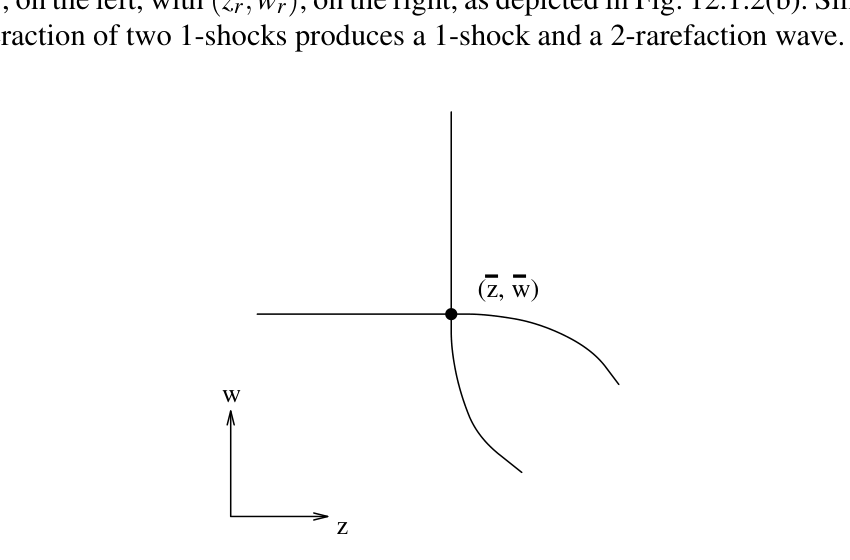
\includegraphics[width=0.55\textwidth]{ch12-fig01-01.png}
\caption{从状态 $(\bar z,\bar w)$ 发出的激波曲线与稀疏波曲线}
\label{figure:ch12-激波稀疏曲线}
\end{figure}

\begin{figure}[ht]
\centering
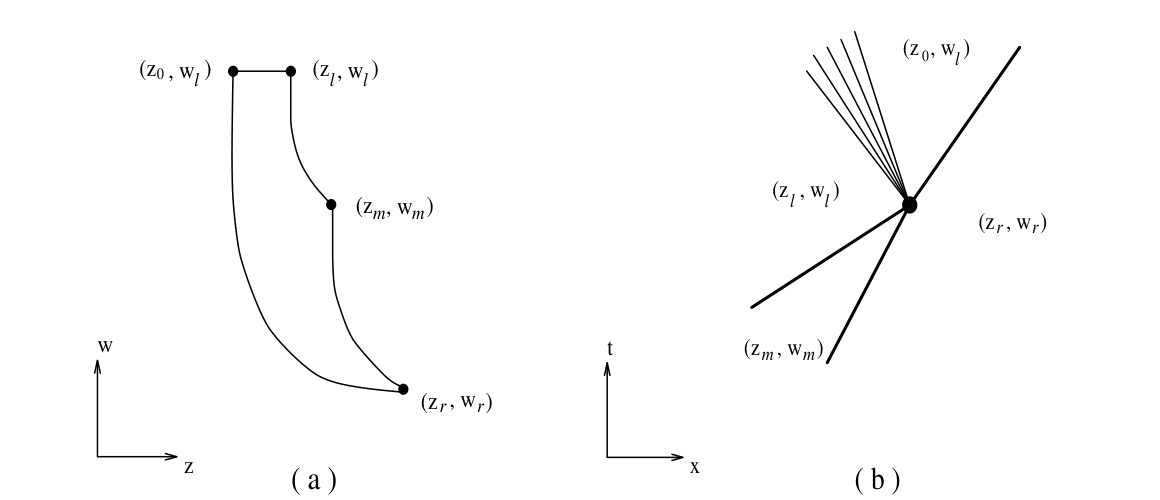
\includegraphics[width=0.95\textwidth]{ch12-fig01-02.png}
\caption{两个 2-激波的相互作用：(a) 状态平面；(b) $(x,t)$ 平面中的波扇}
\label{figure:ch12-激波相互作用}
\end{figure}

同样为确定起见，我们假设
\begin{align}
\lambda_w<0,\qquad \mu_z>0,
\label{align:ch12-混合导数}
\end{align}
或等价地，由原书 (7.3.14) 与 (7.4.15)，
\begin{align}
R^{\top}\mathrm{D}^2_z S>0,\qquad S^{\top}\mathrm{D}^2_w R>0.
\label{align:ch12-混合二阶}
\end{align}
典型的例子是等温热弹性的系统原书 (7.1.11)，它满足\eqref{align:ch12-真非线性}、\eqref{align:ch12-相互作用} 与\eqref{align:ch12-混合二阶}全部三个假设，并以原书 (7.3.2) 为 Riemann 不变量，只要 $\sigma''(u)<0$，即弹性介质为软弹簧或气体。
当介质为硬弹簧，即 $\sigma''(u)>0$ 时，原书 (7.3.2) 中 Riemann 不变量的符号必须反向。

\end{document}
